In this part, we have implemented five different integration methods to compute the length of plane curves defined by an integral. The objective is to optimize the measurement of the curves by choosing the appropriate method in terms of speed and convergence.
Selecting the right integration method is crucial for achieving accurate and efficient results. Therefore, we have tested and compared the performance of each method to determine which one is most suitable for our application.
\subsection{Integration methods}
Let $ f : [a,b] \rightarrow \mathbb{R} $, $n$ the number of intervals with $a = x_{0} < x_{1}< ...<x_{n} = b$ and $ h = x_{i+1} -x{i}$ the constant length of intervals.
\paragraph{left and right rectangle method}
The rectangle approximation method consists on dividing the area under a curve into multiple rectangles with small widths. This method is based on the Riemann integral definition and assumes that the widths of the rectangles are constant.
When computing a Riemann sum, the method for positioning the rectangles is important. One possibility is to align the rectangles such that their top-left corners touch the curve, which is referred to as a left Riemann sum given by $\int_{a}^{b}f(x)dx =  h\sum_{k=0}^{k=n-1} f(x_{k}) $.
Another approach is to place the rectangles such that their top-right corners touch the curve, known as a right Riemann sum and given by $\int_{a}^{b}f(x)dx =  h\sum_{k=1}^{k=n} f(x_{k}) $.
\paragraph{middle point method}
The middle point method is another option of the rectangle approximation which involves aligning the rectangles such that their midpoints touch the curves. This method is implemented by the following formula $\int_{a}^{b}f(x)dx =  h\sum_{k=1}^{k=n} f(\frac{x_{i-1} -x{i}}{2})$.
\paragraph{Trapezoidal method}
The trapezoidal method is a numerical integration technique that approximates the area under a curve by dividing the region into multiple trapezoids, rather than rectangles as in the rectangle method. By summing up the areas of all the trapezoids, we can obtain an estimation of the integral. Unlike the rectangle method, the trapezoidal method considers the slope of the curve between each pair of adjacent points by using a linear interpolation, which results in a more accurate approximation. The formula for trapezoidal method is :
$\int_{a}^{b}f(x)dx  = \frac{h}{2}(f(a) + f(b)) + h\sum_{k=1}^{k=n} f(x_{k}) = I_{h}$

\paragraph{Simpson method}
Simpson's method is a numerical integration technique that approximates the area under a curve by dividing the region into an even number of subintervals and fitting a second-degree polynomial to each pair of consecutive points on the curve. By computing the area under each parabolic segment and summing them up, we can obtain an estimation of the integral. Simpson's method is known to be more accurate than the rectangle and trapezoidal methods, especially for curves that are quadratic or less, as it can provide exact results in such cases. The formula for Simpson's method is : \\
$\int_{a}^{b}f(x)dx = \frac{h}{6}(f(a)+f(b)) +\frac{2h}{3}\sum_{k=0}^{k=n-1}f(x_{i} +\frac{h}{2})  + \frac{h}{3}\sum_{k=0}^{k=n-1} f(x_{i}) = \frac{4}{3}I_{\frac{h}{2}} - \frac{1}{3}I_{h} $ \\
with $I_{h}$ the trapezoidal approximation of $\int_{a}^{b}f(x)dx $ using $\frac{a-b}{h}$ interval.

\subsection{Convergence analysis}
\label{section}
Once we validated the different integration methods on various polynomial and non-polynomial functions, we proceeded to analyze their convergence for a specific polynomial integral $ I = \int_{0}^{2}(x^{3} -3x +2)dx$. To do so, we evaluated the integral approximation for different values of the number $N$ of intervals, and studied how the accuracy of the approximation improved as we increased $N$. \\
According to Figure \ref{fig:speed}, the Simpson's method displays a faster convergence than the trapezoidal and rectangle methods. In fact, for $N=10$, the Simpson's method achieves an error of about $10^{-16}$, while the trapezoidal method yields an error of $0.04$, and the midpoint method yields an error of $0.01$. On the other hand, the left and right rectangle methods converge much more slowly.These results could be justified by the fact that the Simpson's method approximates the curve with quadratic polynomials, while the other methods use linear approximations.\\
\begin{figure}[H]
  \label{fig:speed}
  \centering
  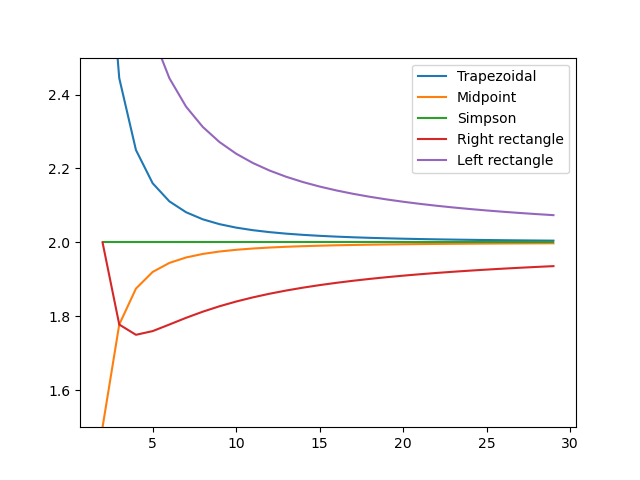
\includegraphics[width=0.8\textwidth]{tex/speed_convergence.png}
  \caption{Approximations of the integral in function of the number $N$ of intervals I using the different methods }  
\end{figure}

\subsection{Length of the plane curves} 
In section~\ref{section}, it was found that the Simpson method is a suitable numerical integration method for approximating the length of splines, as it provides fast convergence and high accuracy. This method can be used to approximate the integral $\int \sqrt{1+f'(x)^{2}}dx$, which is used to determine the length of the spline.

To approximate the derivative of the function f, we utilized the central difference formula $f'(x) = \frac{f'(x+h) - f'(x-h)}{2h}$, which uses the values of the function at points slightly to the left and right of the point at which the derivative is being approximated. This formula has an error of order 2, which means that the accuracy of the approximation improves as the step size h becomes smaller.


